\chapter{Aspectos Conceituais} \label{cap:conceitos}


A proteção efetiva de um sistema não é alcançada por uma única técnica, 
mas pela combinação de estratégias em múltiplas camadas. Conforme o 
\textit{NIST Cybersecurity Framework} \cite{nist_csf_2024}, a segurança 
robusta exige tanto \textbf{prevenção} (impedindo que ataques ocorram) 
quanto \textbf{detecção} (identificando atividades suspeitas). Este 
capítulo apresenta os conceitos que fundamentam este trabalho dentro 
desse paradigma: protocolos de comunicação para IoT, criptografia leve 
como mecanismo preventivo, e Machine Learning como mecanismo de detecção 
comportamental.


\section{Redes IoT e o Protocolo LoRaWAN}

As redes de Internet das Coisas (IoT) utilizam amplamente o protocolo LoRaWAN em cenários que exigem baixo consumo de energia e ampla cobertura. Embora o LoRaWAN apresente certa maturidade e conte com mecanismos de proteção continuamente aprimorados, ataques e problemas de segurança ainda afetam sua resiliência. Consequentemente, permanece necessária a evolução contínua de técnicas de prevenção e mitigação dessas ameaças \cite{hessel2023lorawan}.

%%%%%%%%%%%%%%%%%%%%%%%%%%%%%%%%%%%%%%%%%%%%%%%%%%%%

\subsection{LoRa e LoRaWAN: fundamentos e evolução do protocolo}

O LoRaWAN se destaca como uma tecnologia voltada a redes LPWAN (\textit{Low-Power Wide-Area Network}), sendo utilizado em aplicações como monitoramento remoto, agricultura inteligente e sistemas distribuídos com dispositivos embarcados. Sua proposta é permitir a comunicação entre dispositivos com baixo consumo energético, ampla cobertura e custo operacional reduzido.

É importante distinguir os termos \textit{LoRa} e \textit{LoRaWAN}, que frequentemente são tratados como sinônimos, embora representem camadas diferentes da tecnologia. O LoRa corresponde à camada física da comunicação, isto é, à técnica de modulação empregada no enlace sem fio. Já o LoRaWAN define o protocolo de comunicação acima dessa camada, estabelecendo regras para organização da rede, troca de mensagens e controle da comunicação. Em outras palavras, o LoRa fornece o meio de transmissão por rádio, enquanto o LoRaWAN define o funcionamento da rede sobre esse meio.

De forma geral, o LoRaWAN foi projetado para redes compostas por dispositivos com recursos limitados, muitas vezes alimentados por bateria e instalados em locais de difícil manutenção. Por isso, o protocolo prioriza simplicidade operacional, baixo consumo e comunicação eficiente, ainda que com taxas de transmissão menores do que tecnologias voltadas a maior vazão de dados. Essa característica o torna adequado para cenários em que pequenas quantidades de informação precisam ser transmitidas periodicamente, sem necessidade de comunicação contínua.

A evolução do LoRaWAN também é um aspecto importante. Desde sua primeira publicação, em 2015, o protocolo passou por revisões que resultaram em dois ramos principais: a família 1.0.x e a versão 1.1. As versões da família 1.0.x mantiveram interoperabilidade entre si e trouxeram principalmente correções, esclarecimentos e ajustes incrementais. Já a versão 1.1 introduziu mudanças mais relevantes, especialmente na organização de funções da rede e nos mecanismos de segurança, tornando mais clara a separação entre responsabilidades de rede e de aplicação.

\begin{figure}[htb]
  \caption{\label{lorawan_version_history}Histórico de versionamento da especificação da LoRaWAN}
  \begin{center}
      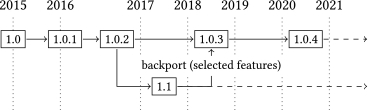
\includegraphics[scale=0.8]{figuras/lorawan_version_history.png}
  \end{center}
  \legend{Fonte: \cite{hessel2023lorawan}}
\end{figure}

Mesmo com a introdução de melhorias nas versões mais recentes, a adoção de novas revisões do protocolo não ocorre de forma imediata em sistemas reais. Em aplicações IoT, sensores podem permanecer em operação por muitos anos, frequentemente sem atualização de firmware. Como consequência, versões anteriores do LoRaWAN continuam relevantes na prática, e essa coexistência entre gerações do protocolo precisa ser considerada em qualquer análise técnica ou experimental.

Assim, compreender a distinção entre LoRa e LoRaWAN, bem como a evolução do protocolo ao longo de suas versões, é essencial para analisar corretamente seu funcionamento em sistemas embarcados conectados. A partir dessa base, as próximas subseções detalham a arquitetura da rede, o processo de ativação dos dispositivos, a transferência de dados, os mecanismos de gerenciamento da comunicação e a relação dessas tecnologias com a arquitetura proposta neste trabalho.

%%%%%%%%%%%%%%%%%%%%%%%%%%%%%%%%%%%%%%%%%%%%%%%%%%%%

\subsection{Arquitetura da Rede}

A arquitetura do LoRaWAN é composta por diferentes entidades, cada uma com uma função específica no funcionamento da rede. De forma geral, os dispositivos finais, chamados de \textit{End Devices}, são responsáveis por coletar e transmitir dados. Esses dispositivos se comunicam por rádio com um ou mais \textit{Gateways}, que atuam como pontes entre a rede LoRa e a infraestrutura conectada por IP. Os gateways, por sua vez, apenas recebem os quadros transmitidos pelos dispositivos e os encaminham para os servidores da rede, sem realizar processamento completo do protocolo. \cite{hessel2023lorawan}

Essa organização forma uma topologia conhecida como \textit{star-of-stars}. Nela, os dispositivos finais não se comunicam diretamente entre si, e também não estabelecem vínculo fixo com um único gateway. Em vez disso, uma mesma transmissão pode ser recebida por vários gateways que estejam dentro de alcance. Essa característica aumenta a cobertura da rede e oferece maior robustez na recepção das mensagens, especialmente em cenários distribuídos e com mobilidade.

\begin{figure}[htb]
  \caption{\label{lorawan_architeture}Arquitetura de rede LoRaWAN}
  \begin{center}
      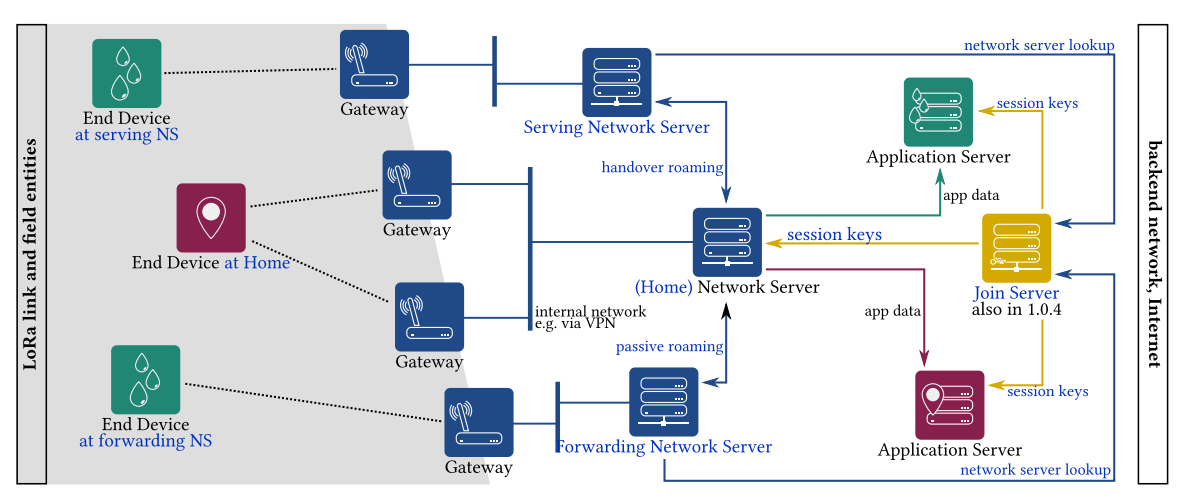
\includegraphics[scale=0.4]{figuras/architeture_LoRaWan.png}
  \end{center}
  \legend{Fonte: \cite{hessel2023lorawan}}
\end{figure}

Após o encaminhamento feito pelos gateways, as mensagens chegam ao \textit{Network Server}. Esse servidor exerce papel central na rede, pois é responsável por processar as mensagens recebidas, eliminar duplicidades causadas pela recepção do mesmo quadro por múltiplos gateways, validar a integridade das mensagens e executar as funções de gerenciamento da camada MAC. Em outras palavras, é o \textit{Network Server} que coordena o funcionamento lógico da rede LoRaWAN.

Os dados de aplicação seguem então para o \textit{Application Server}, que é o componente responsável por tratar a informação útil transportada pelo dispositivo final. É nesse servidor que os dados recebidos podem ser decifrados, interpretados e encaminhados para a aplicação de interesse, como um sistema de monitoramento, um banco de dados ou uma plataforma de análise. Essa separação entre funções de rede e funções de aplicação é importante porque organiza melhor as responsabilidades do sistema e reduz o acoplamento entre comunicação e processamento da informação.

Na evolução do protocolo, especialmente a partir do LoRaWAN 1.1, o \textit{Join Server} passa a ter um papel mais explícito na arquitetura. Esse componente participa do processo de ativação dos dispositivos e da derivação de chaves de sessão, contribuindo para uma separação mais clara entre gerenciamento de rede e segurança da aplicação. Com isso, a arquitetura do LoRaWAN se torna mais organizada do ponto de vista funcional e mais adequada a cenários em que diferentes operadores ou domínios de serviço precisam cooperar.

Assim, a arquitetura do LoRaWAN pode ser entendida como uma organização em camadas funcionais: o dispositivo final coleta e transmite os dados, o gateway encaminha os quadros recebidos, o \textit{Network Server} gerencia a comunicação da rede, e o \textit{Application Server} entrega os dados à aplicação. Nas versões mais recentes, o \textit{Join Server} complementa essa estrutura ao apoiar o processo de ativação e gerenciamento de chaves. Essa divisão de papéis é fundamental para compreender como o protocolo opera e como seus componentes podem ser relacionados à arquitetura proposta neste trabalho.

%%%%%%%%%%%%%%%%%%%%%%%%%%%%%%%%%%%%%%%%%%%%%%%%%%%%

\subsection{Ativação do Dispositivo}

Antes de transmitir dados de aplicação, um dispositivo LoRaWAN precisa ser ativado na rede. Esse processo define como o dispositivo passa a ser reconhecido pelo sistema e como obtém o contexto necessário para a comunicação, incluindo identificadores, parâmetros de sessão e chaves utilizadas ao longo da operação. De forma geral, o LoRaWAN admite dois modos principais de ativação: \textit{Activation By Personalization} (ABP) e \textit{Over-The-Air Activation} (OTAA). \cite{hessel2023lorawan}

No modo ABP, o dispositivo já é configurado previamente com os parâmetros de sessão necessários para operar. Assim, ele pode iniciar a transmissão diretamente, sem realizar um procedimento de ingresso na rede a cada inicialização. Essa abordagem é mais simples do ponto de vista de implementação, mas oferece menor flexibilidade operacional, já que os parâmetros de comunicação ficam previamente fixados no dispositivo.

No modo OTAA, por outro lado, o dispositivo realiza um procedimento de ingresso na rede antes de iniciar sua operação normal. Nesse processo, o nó envia uma solicitação de ativação e, a partir da resposta da infraestrutura da rede, passa a operar com parâmetros e chaves de sessão derivados especificamente para aquela conexão. Em comparação com o ABP, essa abordagem é mais flexível e mais adequada a cenários reais, pois facilita renovação de chaves, adaptação do contexto de comunicação e suporte a funcionalidades mais avançadas do protocolo.

De forma simplificada, a ativação por OTAA envolve a troca de mensagens de ingresso e a geração de chaves de sessão a partir de credenciais previamente associadas ao dispositivo. Esse mecanismo permite que a rede estabeleça uma nova sessão de comunicação de forma controlada, em vez de depender sempre de parâmetros estáticos. Por esse motivo, o OTAA tende a ser considerado a alternativa mais robusta para implantações práticas, especialmente quando se deseja maior controle do ciclo de vida dos dispositivos e melhor suporte a segurança.

\begin{figure}[htb]
  \caption{\label{lorawan_join_process} (a) OTAA processo de entrada LoRaWAN 1.0.x. (b) OTAA processo de entrada LoRaWAN 1.1}
  \begin{center}
      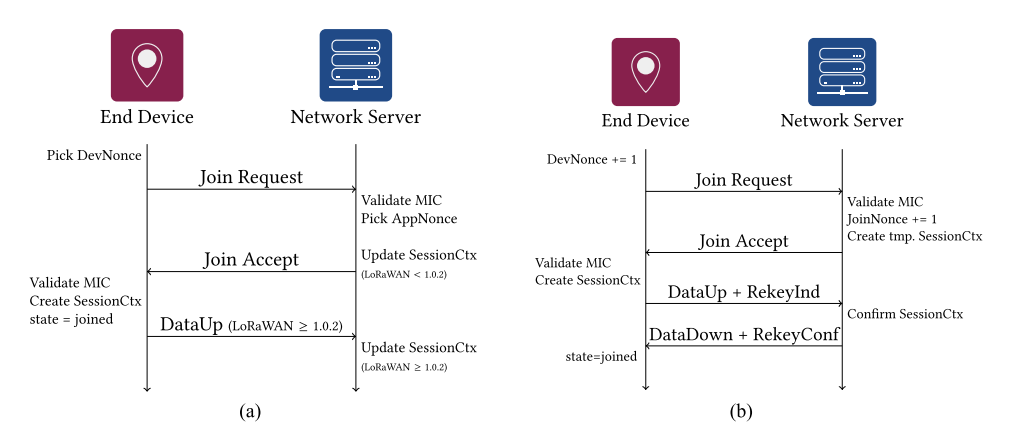
\includegraphics[scale=0.4]{figuras/otaa_join_process.png}
  \end{center}
  \legend{Fonte: \cite{hessel2023lorawan}}
\end{figure}

A evolução do protocolo também impacta esse processo. Nas versões da família 1.0.x, a ativação já podia ocorrer por ABP ou OTAA, mas a versão 1.1 introduziu uma separação mais clara entre funções de rede e aplicação, além de mudanças no tratamento das chaves e no papel do \textit{Join Server}. Com isso, o processo de ativação passou a ser mais estruturado e alinhado com uma arquitetura de segurança mais organizada.

Assim, a ativação do dispositivo representa uma etapa fundamental no funcionamento do LoRaWAN, pois estabelece as condições iniciais para que a comunicação ocorra de forma válida dentro da rede. Enquanto o ABP oferece uma alternativa mais simples, o OTAA apresenta maior flexibilidade e melhor aderência a cenários práticos e escaláveis. A partir dessa etapa, o dispositivo pode iniciar a troca de dados com a infraestrutura da rede, conforme discutido na próxima subseção.

%%%%%%%%%%%%%%%%%%%%%%%%%%%%%%%%%%%%%%%%%%%%%%%%%%%%

\subsection{Transferência de Dados}

Após a ativação do dispositivo, a comunicação de dados pode ocorrer entre o dispositivo final e a infraestrutura da rede. No LoRaWAN, as mensagens enviadas pelo dispositivo em direção à rede são chamadas de \textit{DataUp}, enquanto as mensagens enviadas pela rede ao dispositivo são chamadas de \textit{Datadown}. Essa troca de dados pode ocorrer de forma simples, apenas com envio da informação, ou com solicitação de confirmação de recebimento, dependendo da necessidade da aplicação. \cite{hessel2023lorawan}

Quando não há necessidade de confirmação, utilizam-se mensagens não confirmadas, que reduzem o overhead da comunicação e tendem a ser mais adequadas a aplicações periódicas de monitoramento. Já nas mensagens confirmadas, a camada MAC pode exigir uma resposta da rede, permitindo ao dispositivo verificar se a transmissão foi reconhecida. Essa distinção é importante porque envolve um compromisso entre confiabilidade e consumo de recursos, já que confirmações adicionais aumentam o uso do canal e o gasto energético.

\begin{figure}[htb]
  \caption{\label{lorawan_message_ed}Classe para comunicacoes ED}
  \begin{center}
      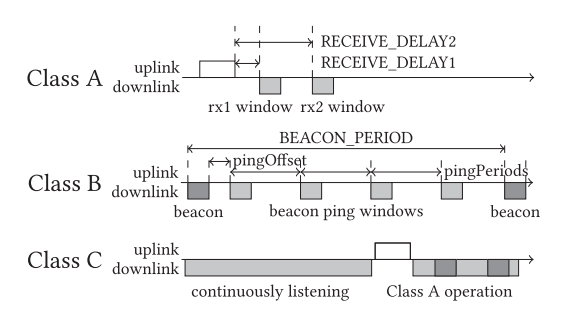
\includegraphics[scale=0.6]{figuras/ed_operations_class.png}
  \end{center}
  \legend{Fonte: \cite{hessel2023lorawan}}
\end{figure}

O LoRaWAN define três modos principais de operação para os dispositivos finais, chamados de classes A, B e C. A Classe A é a padrão e está presente em todos os dispositivos LoRaWAN. Nela, o dispositivo inicia a comunicação por meio de um \textit{uplink} e, após essa transmissão, abre duas pequenas janelas de recepção para possíveis mensagens de \textit{downlink}. Essas janelas são conhecidas como RX1 e RX2. Esse modelo é o mais eficiente em termos energéticos, pois o dispositivo permanece a maior parte do tempo fora de escuta. 

Na Classe B, além do comportamento básico da Classe A, o dispositivo sincroniza sua operação com sinais periódicos da rede e passa a abrir janelas adicionais de recepção em instantes programados. Isso permite maior previsibilidade para o envio de mensagens em \textit{downlink}, embora aumente a complexidade da operação. Já na Classe C, o dispositivo permanece praticamente em escuta contínua, fechando a recepção apenas quando transmite. Essa abordagem reduz a latência de \textit{downlink}, mas aumenta significativamente o consumo de energia, sendo mais adequada a dispositivos com menor restrição energética.

\begin{figure}[htb]
  \caption{\label{messages_abc} Estrutura e Criptografia das mensagems LoRaWan}
    \begin{center}
      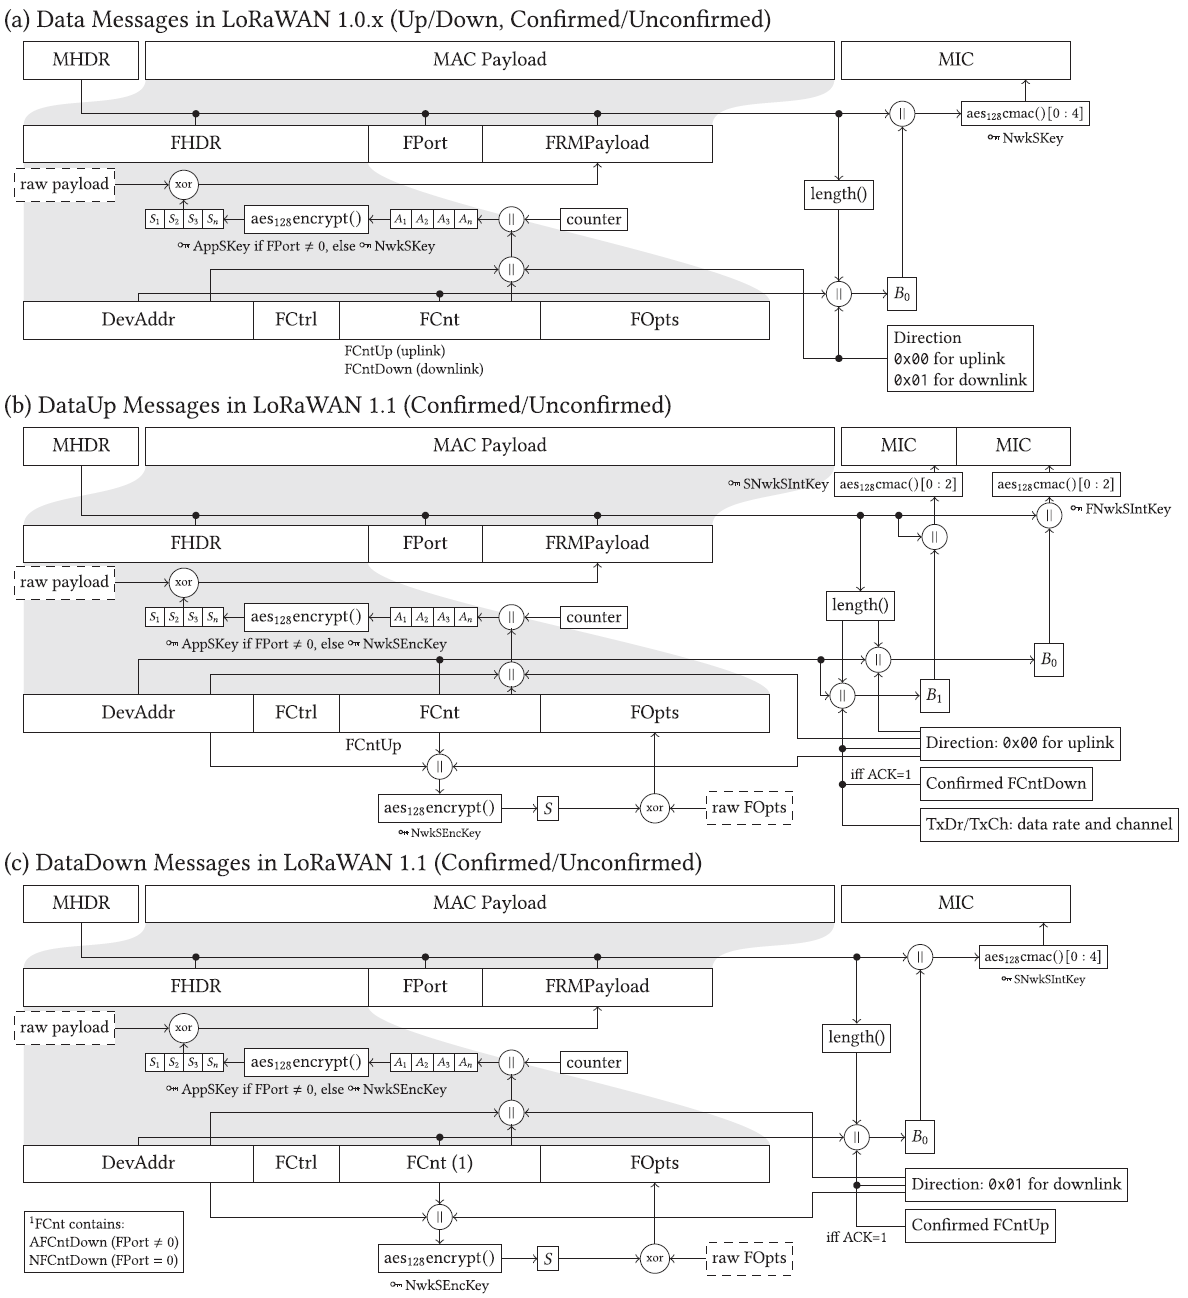
\includegraphics[scale=0.3]{figuras/structure_messages_abc.png}
  \end{center}
  \legend{Fonte: \cite{hessel2023lorawan}}
\end{figure}

As mensagens de dados do LoRaWAN possuem uma estrutura padronizada. De forma geral, elas incluem um cabeçalho com a identificação do tipo de mensagem, um cabeçalho de quadro com informações de controle e endereçamento, um contador de quadros e o campo destinado à carga útil da aplicação. Entre esses elementos, o contador de quadros, representado por \textit{FCnt}, é especialmente importante para o acompanhamento da sequência das mensagens. Outros campos, como \textit{FPort} e \textit{FOpts}, ajudam a distinguir dados de aplicação e informações de controle da rede. Além disso, as mensagens incluem um código de integridade, chamado \textit{MIC}, utilizado para verificação da validade da comunicação.

De modo geral, a transferência de dados no LoRaWAN foi projetada para equilibrar simplicidade, baixo consumo e capacidade de operação em redes distribuídas de longo alcance. A existência de diferentes classes de operação e de mecanismos para mensagens confirmadas ou não confirmadas permite adaptar o comportamento da comunicação às necessidades da aplicação. A partir dessa base, torna-se possível compreender melhor como a rede ajusta e gerencia sua operação, tema discutido na próxima subseção.

%%%%%%%%%%%%%%%%%%%%%%%%%%%%%%%%%%%%%%%%%%%%%%%%%%%%

\subsection{Gerenciamento da Rede}

Como o LoRaWAN é um protocolo de camada MAC voltado a redes LPWAN, ele precisa de mecanismos para configurar dispositivos, ajustar parâmetros de comunicação e acompanhar o estado da rede. Parte dessas funções já aparece diretamente nos próprios campos das mensagens, como endereços, contadores de quadros e confirmações. No entanto, o protocolo também define comandos específicos para gerenciamento, conhecidos como \textit{MAC commands}, que permitem trocar informações de controle entre o dispositivo final e a infraestrutura da rede. \cite{hessel2023lorawan}

Esses comandos são usados para diferentes finalidades de operação. Entre elas, estão a obtenção de informações sobre a qualidade da conexão, o ajuste de parâmetros de transmissão e a sincronização de tempo. Assim, o gerenciamento da rede não ocorre como uma função separada do restante do protocolo, mas sim como parte do próprio fluxo de comunicação entre os dispositivos e os servidores da rede. 

Entre os mecanismos de gerenciamento, um dos mais importantes é o \textit{Adaptive Data Rate} (ADR). O ADR tem como objetivo ajustar a taxa de transmissão de dados e outros parâmetros de rádio de acordo com as condições de comunicação observadas na rede. Na prática, isso permite definir combinações mais adequadas de \textit{Spreading Factor}, largura de banda e potência de transmissão, buscando equilibrar confiabilidade, consumo de energia e uso eficiente do meio de comunicação.

De forma geral, o gerenciamento da rede no LoRaWAN existe para manter a comunicação funcional e eficiente ao longo do tempo. Por meio de comandos de controle e mecanismos como o ADR, o protocolo consegue ajustar seu comportamento às condições reais de operação, o que é especialmente importante em ambientes distribuídos, sujeitos a variações de alcance, interferência e disponibilidade energética. Com essa base conceitual, torna-se possível avançar para uma análise mais voltada à forma como essas tecnologias serão utilizadas na arquitetura proposta neste trabalho.

%%%%%%%%%%%%%%%%%%%%%%%%%%%%%%%%%%%%%%%%%%%%%%%%%%%%

\subsection{LoRaWAN versus Wi-Fi no contexto do projeto}

Embora LoRaWAN e Wi-Fi sejam tecnologias de comunicação sem fio, elas atendem a necessidades diferentes e, neste trabalho, não são tratadas como soluções concorrentes. Cada uma delas ocupa um papel específico na arquitetura proposta, de acordo com suas características de alcance, consumo energético, taxa de transmissão e facilidade de integração com os demais componentes do sistema.

O LoRaWAN foi pensado para aplicações de longo alcance e baixo consumo, sendo mais adequado a dispositivos embarcados que operam com recursos limitados e transmitem pequenas quantidades de dados de forma periódica ou eventual. Essas características o tornam compatível com o cenário deste projeto, no qual os nós sensores e atuadores precisam operar de forma eficiente, com comunicação sem fio e possibilidade de instalação em locais mais afastados do ponto central da rede.

O Wi-Fi, por outro lado, oferece maior taxa de transmissão e integração mais direta com redes IP e serviços de aplicação, como APIs e servidores de armazenamento. Em contrapartida, apresenta maior consumo energético e menor adequação a nós distribuídos que precisem operar por longos períodos com restrição de energia. Por esse motivo, o Wi-Fi não foi adotado como tecnologia principal de comunicação entre os nós embarcados e a infraestrutura de campo.

No contexto deste trabalho, a solução adotada combina as duas tecnologias de forma complementar. O trecho entre os nós sensores/atuadores e o gateway utiliza LoRaWAN, preservando as vantagens de alcance e baixo consumo no nível embarcado. Já o trecho entre o gateway e o servidor utiliza Wi-Fi, aproveitando sua integração mais simples com a infraestrutura de rede e com os serviços responsáveis por receber, armazenar e processar os dados coletados.

Essa divisão permite separar dois problemas distintos dentro da arquitetura. O primeiro é a comunicação entre dispositivos embarcados em campo, em que baixo consumo e cobertura são requisitos centrais. O segundo é a entrega dos dados para uma camada de processamento e persistência, em que a prioridade passa a ser conectividade com a rede local ou com a Internet, além da facilidade de integração com a aplicação. Assim, a escolha conjunta de LoRaWAN e Wi-Fi não representa uma sobreposição de tecnologias, mas sim uma composição coerente entre camadas com funções diferentes.

Dessa forma, o uso de LoRaWAN no trecho embarcado e de Wi-Fi no trecho de retaguarda estabelece uma arquitetura compatível com os objetivos do projeto. Ao mesmo tempo em que preserva as vantagens de uma rede LPWAN na comunicação entre os dispositivos de campo, essa abordagem também facilita a construção da interface com o servidor, a persistência dos dados e a futura integração com mecanismos de análise e segurança.

%%%%%%%%%%%%%%%%%%%%%%%%%%%%%%%%%%%%%%%%%%%%%%%%%%%%

\subsection{Implicações para a arquitetura proposta}

Os conceitos apresentados nas subseções anteriores permitem situar a arquitetura adotada neste trabalho. No projeto proposto, os nós sensores e atuadores operam como dispositivos finais responsáveis pela coleta de dados do ambiente e pela transmissão dessas informações pela rede sem fio. Essa comunicação ocorre no trecho embarcado por meio do LoRaWAN, explorando suas características de longo alcance e baixo consumo energético.

O gateway exerce o papel de ponto de transição entre a rede de campo e a infraestrutura de retaguarda. Sua função principal é receber os quadros enviados pelos dispositivos finais e encaminhá-los para a camada de processamento do sistema. A partir desse ponto, os dados podem ser entregues a um servidor ou API responsável por armazenamento, organização e disponibilização das informações para etapas posteriores de análise.

Essa divisão é importante porque separa o problema da comunicação embarcada do problema de processamento dos dados. No nível dos nós em campo, o foco está em transmitir com eficiência, respeitando restrições de energia, alcance e capacidade computacional. Já no nível do gateway e do servidor, torna-se possível concentrar funções de persistência, observabilidade e integração com serviços de aplicação, sem impor esse custo diretamente aos dispositivos finais.

Entretanto, o uso do LoRaWAN por si só não elimina todos os desafios de segurança do sistema. Como discutido na literatura, a proteção efetiva da rede depende não apenas do protocolo, mas também da forma como seus mecanismos são implementados e integrados à aplicação. Em particular, a presença de dados trafegando entre dispositivos embarcados, gateway e infraestrutura de backend torna necessário considerar mecanismos adicionais de proteção, especialmente quando o sistema opera em ambientes distribuídos e sujeitos a diferentes tipos de ameaça.

Além disso, a própria dinâmica operacional da rede produz informações que podem ser úteis para análise de comportamento, identificação de falhas e detecção de atividades anômalas. Parâmetros de transmissão, padrões temporais de envio e eventos observados na comunicação podem servir como base para uma camada adicional de monitoramento do sistema, complementando a proteção oferecida pelos mecanismos tradicionais do protocolo.

Dessa forma, a arquitetura proposta neste trabalho não se limita ao transporte de dados entre dispositivos e servidor. Ela também cria as condições para incorporar camadas complementares de segurança e análise. Nesse contexto, a próxima seção discute o uso de criptografia leve como mecanismo adequado à proteção de dados em dispositivos com recursos restritos, enquanto a seção seguinte apresenta o papel do \textit{Machine Learning} como apoio à análise do comportamento da rede e à detecção de anomalias.


%%%%%%%%%%%%%%%%%%%%%%%%%%%%%%%%%%%%%%%%%%%%%%%%%%%%
%%%%%%%%%%%%%%%%%%%%%%%%%%%%%%%%%%%%%%%%%%%%%%%%%%%%

\section{Criptografia Leve (Lightweight Cryptography) e o Padrão Ascon}
Em dispositivos IoT, onde o baixo consumo de energia é um requisito essencial para viabilizar operações em diversas áreas, as aplicações que lidam com dados sensíveis e exigem sigilo demandam a adoção de métodos criptográficos que sejam, simultaneamente, leves e seguros.

O Instituto Nacional de Padrões e Tecnologia dos Estados Unidos (NIST) atua, desde 1973, no desenvolvimento de normas para proteger dados sensíveis transmitidos entre dispositivos. Seu histórico abrange desde a criação do \textit{Data Encryption Standard} (DES) e a consolidação do atual padrão de criptografia simétrica, o \textit{Advanced Encryption Standard} (AES), até as recentes padronizações de criptografia pós-quântica (\textit{Post-Quantum Cryptography}) e de criptografia leve (\textit{Lightweight Cryptography}) \cite{chen2022cornerstone}.

Com o crescimento expressivo do uso de dispositivos IoT, a necessidade de estabelecer um padrão robusto de criptografia leve tornou-se urgente. Isso impulsionou o desenvolvimento de uma nova padronização internacional com o objetivo de contemplar as primitivas criptográficas e os modos de operação adequados para ambientes restritos. Os critérios exigidos para esse novo padrão incluíam resiliência de segurança, flexibilidade de implementação, baixa sobrecarga ao integrar múltiplas funções e proteção intrínseca contra ataques de canal lateral (\textit{Side-Channel Attacks}), entre outros requisitos técnicos \cite{nistir8114}.

O processo de padronização promovido pelo NIST ocorreu ao longo de múltiplas fases de testes e escrutínio público. Inicialmente, 57 algoritmos foram submetidos para consideração. Desses, 32 avançaram para a segunda rodada e, após rigorosas avaliações de desempenho e segurança, apenas 10 chegaram à fase final. A culminação desse extenso projeto ocorreu, em 2023, com o anúncio da família Ascon como a grande vencedora \cite{ascon_official}.

O desenvolvimento do padrão Ascon começou em 2014 e ele será o foco principal deste trabalho. Na prática, ele funciona como um conjunto de algoritmos construído sob medida para dispositivos com poucos recursos. A padronização oficial conta com quatro variações principais. A primeira delas é o Ascon-AEAD128, que criptografa os dados, verifica a autenticidade da mensagem e oferece uma boa proteção contra ataques de canal lateral. A segunda variação é o Ascon-Hash256, criado especificamente para garantir a integridade dos dados transmitidos pela rede. Por fim, existem o Ascon-XOF128 e o Ascon-CXOF128. Ambos funcionam como funções de saída extensível, uma característica que permite ajustar o tamanho do \textit{hash} gerado e economizar recursos computacionais durante o processamento \cite{nist2025ascon}.

%%%%%%%%%%%%%%%%%%%%%%%%%%%%%%%%%%%%%%%%%%%%%%%%%%%%

\subsection{O Padrão Ascon-AEAD128}
O algoritmo de criptografia autenticada escolhido para o projeto pertence à família Ascon, padronizada pelo NIST sob a forma do Ascon-AEAD128 \citeonline{nist2025ascon}. Na prática, a implementação adotada neste trabalho utiliza a variante Ascon-128a, finalista do processo de padronização (versão 1.2), que compartilha a mesma estrutura de permutação do algoritmo padronizado, conforme detalhado na Seção \ref{subsec:biblioteca-ascon}. A utilização de funções de \textit{hash} adicionais não será necessária, uma vez que esse algoritmo já garante confidencialidade, integridade e autenticidade em uma única operação de criptografia autenticada.

O processo de encriptação do Ascon-AEAD128 recebe como entrada uma chave secreta e um \textit{nonce}, ambos de 128 bits, além dos dados associados (\textit{Associated Data} - AD) e o texto em claro a ser cifrado (\textit{plaintext}), que possuem tamanhos variáveis. A saída dessa função é o texto cifrado (\textit{ciphertext}) acompanhado de uma \textit{Tag} de Autenticação de 128 bits. Por sua vez, a função de decriptação recebe a chave, o \textit{nonce}, os dados associados, o texto cifrado e a \textit{tag} de autenticação. O texto original em claro só é retornado se a \textit{tag} for validada com sucesso. Caso contrário, a operação é abortada e retorna um erro (\textit{fail}).

O estado interno inicial de ambos os processos possui 320 bits, sendo formado pela concatenação de 64 bits do Vetor de Inicialização (IV), 128 bits da chave secreta e 128 bits do \textit{nonce}. Após a inicialização, o algoritmo segue em fases: primeiro ocorre o processamento dos dados associados (se presentes), seguido pela cifração do texto em blocos e, ao final de todo o processamento, a fase de finalização gera a \textit{tag} de autenticação.

\begin{figure}[htb]
  \caption{\label{fluxo-ascon-aead128-encript}Processo de encriptação do Ascon-AEAD128}
  \begin{center}
    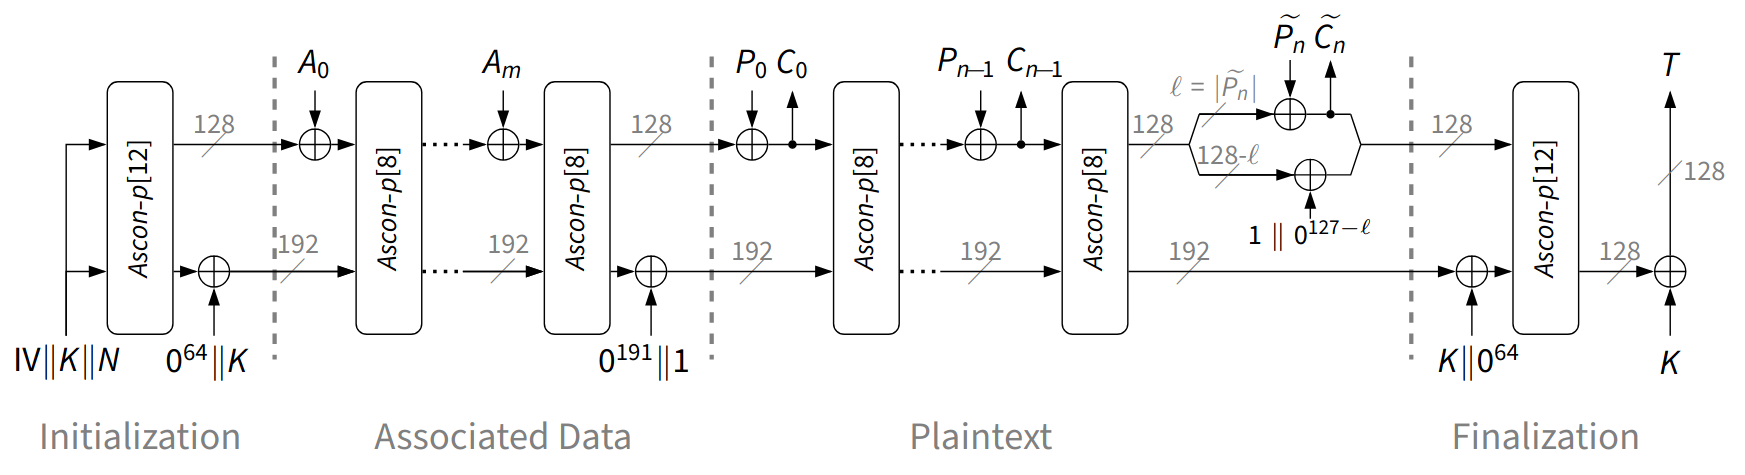
\includegraphics[scale=0.25]{figuras/fluxo-ascon-aead128-encript.png}
  \end{center}
  \legend{Fonte: \cite{nist2025ascon}}
\end{figure}

O processo de decriptação possui uma estrutura muito semelhante à da encriptação. Ele passa pela mesma inicialização do estado de 320 bits e pelo processamento dos dados associados. A diferença principal ocorre nas etapas finais: o texto cifrado é processado bloco a bloco para recuperar o texto original e, na fase de finalização, a chave secreta é combinada com o estado interno para recalcular a \textit{tag} de autenticação. Se a \textit{tag} recalculada for idêntica à \textit{tag} recebida, o texto decifrado é considerado autêntico e é retornado, caso contrário, a mensagem é descartada.

\begin{figure}[htb]
  \caption{\label{fluxo-ascon-aead128-dencript}Processo de dencriptação do Ascon-AEAD128}
  \begin{center}
    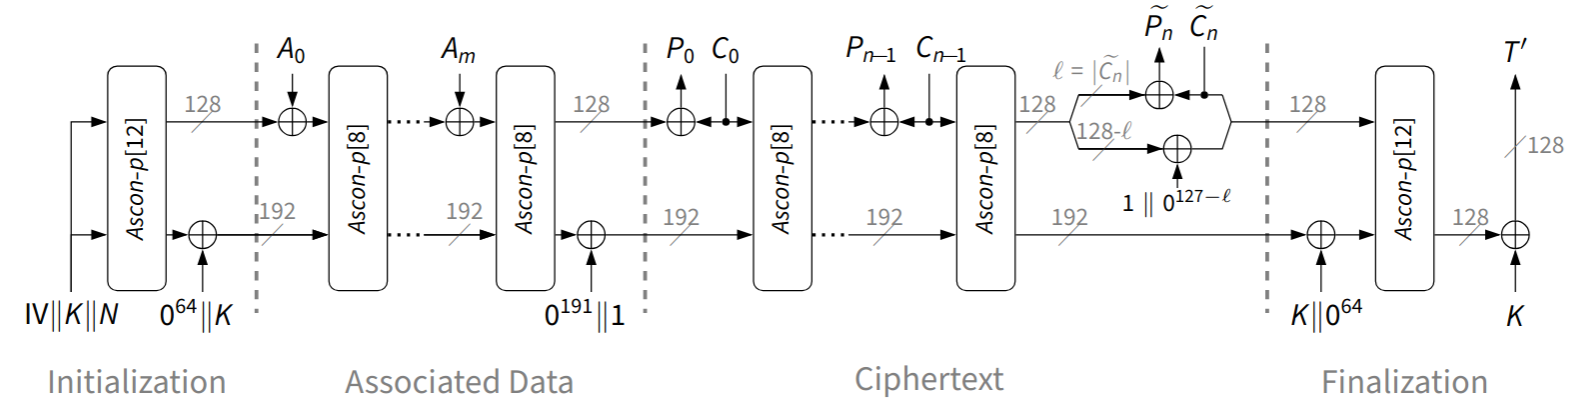
\includegraphics[scale=0.35]{figuras/fluxo-ascon-aead128-decript.png}
  \end{center}
  \legend{Fonte: \cite{nist2025ascon}}
\end{figure}

%%%%%%%%%%%%%%%%%%%%%%%%%%%%%%%%%%%%%%%%%%%%%%%%%%%%

\subsection{Comparativo de Algoritmos Criptográficos para IoT}
Durante a pesquisa inicial sobre criptografia leve, outros algoritmos foram avaliados, mas nenhum se mostrou tão adequado às necessidades do projeto quanto o padrão Ascon. Entre as principais alternativas analisadas, destacam-se o Speck \citeonline{baldi_speck} e o ChaCha20 \citeonline{bernstein2008chacha}. No entanto, a análise aprofundada revelou que nenhum destes se adequava às premissas metodológicas e práticas do projeto quanto o padrão Ascon e as soluções nativas em hardware.

O Speck é uma cifra de bloco pura e bastante leve. No entanto, ele possui uma limitação estrutural importante para redes modernas: não oferece Criptografia Autenticada com Dados Associados (\textit{AEAD}) de forma nativa. Para garantir a integridade da mensagem, seria necessária a adição de um algoritmo de autenticação secundário e independente (como um código de autenticação de mensagem, MAC). O Speck teve sua padronização internacional ativamente rejeitada pela ISO (\textit{International Organization for Standardization}) por falta de transparência em seu design \cite{register2018nsa}.

O ChaCha20, por sua vez, é uma cifra de fluxo de altíssimo desempenho, amplamente adotada como padrão da indústria para cenários de software onde \textbf{não} há aceleração de hardware disponível. Contudo, assim como o Speck, ele carece de propriedades \textit{AEAD} embutidas. A exigência extra de se acoplar o algoritmo Poly1305 consome memória e processamento. Como o microcontrolador utilizado neste trabalho (família ESP32) possui aceleração criptográfica nativa para AES, o cenário de uso principal do ChaCha20 perde o sentido prático.

Para a análise comparativa de viabilidade, este trabalho também optou por não focar nos demais algoritmos finalistas do processo de padronização do NIST (como TinyJAMBU ou Xoodyak) \citeonline{nist_lwc_finalists}, uma vez que a superioridade do Ascon sobre seus pares já foi exaustivamente documentada e comprovada pelo próprio comitê no relatório oficial NIST IR 8454 \cite{nistir8454}.

Dessa forma, a metodologia de comparação deste trabalho foi refinada para responder à questão prática sobre o embate entre o novo padrão de software e o padrão legado de hardware. Os testes focarão exclusivamente em comparar o Ascon (novo padrão \textit{Lightweight Cryptography} do NIST) contra o AES com modo de operação autenticado (\textit{AES-GCM} ou \textit{AES-CCM}) rodando diretamente no coprocessador de hardware do microcontrolador. Essa abordagem permite avaliar se a migração para a criptografia leve em software traz vantagens reais de consumo, memória e latência frente ao uso do acelerador de silício já embutido nas placas comerciais utilizadas em redes \textit{LoRaWAN}.

%%%%%%%%%%%%%%%%%%%%%%%%%%%%%%%%%%%%%%%%%%%%%%%%%%%%
%%%%%%%%%%%%%%%%%%%%%%%%%%%%%%%%%%%%%%%%%%%%%%%%%%%%

\section{Machine Learning}

O uso de \textit{Machine Learning} é coerente com o estado da arte recente. 
Trabalhos como \cite{farhad2023} demonstram que Machine Learning em 
LoRaWAN vem sendo explorado para otimizar parâmetros de rede 
(\textit{spreading factor}, potência de transmissão) e classificar padrões 
de mobilidade.

 Embora parte significativa da literatura esteja concentrada em 
desempenho e eficiência, esse mesmo conjunto de atributos também é 
extremamente relevante para tarefas de segurança e detecção de anomalias, 
já que comportamentos suspeitos frequentemente se refletem justamente em 
mudanças desses padrões operacionais \cite{farhad2023, vangelista2023}.

%%%%%%%%%%%%%%%%%%%%%%%%%%%%%%%%%%%%%%%%%%%%%%%%%%%%

\subsection{Detecção de Anomalias como Problema de Regressão Temporal}

Em redes LoRaWAN operando em condições reais, os dispositivos finais 
transmitem mensagens de forma periódica ou orientada a evento, produzindo 
naturalmente sequências de observações ao longo do tempo. Grandezas como a 
intensidade do sinal recebido, a relação sinal-ruído e os contadores de 
quadros variam de forma contínua e apresentam padrões de comportamento 
relativamente estáveis durante a operação normal da rede. Assim, desvios 
abruptos ou sistemáticos nesses padrões podem indicar a presença de falhas, 
interferências ou atividades maliciosas, tornando a análise temporal dessas 
variáveis uma abordagem promissora para a detecção de anomalias.

No entanto, a aplicação de técnicas supervisionadas de classificação enfrenta 
uma limitação estrutural importante nesse contexto. Em ambientes de operação 
real, dados rotulados que identifiquem explicitamente quadros legítimos e 
quadros associados a ataques são menos presentes.

 O \textit{dataset} Tour Perret, 
utilizado neste trabalho, é representativo da condição: trata-se de um 
conjunto de dados proveniente de sensores reais instalados na Tour Perret, 
em Grenoble, que registra o comportamento contínuo da rede sem a presença 
de rótulos de ataque. Essa característica inviabiliza a utilização direta 
de classificadores supervisionados e exige uma abordagem metodológica 
distinta - o aprendizado de padrões esperados. Mas devido a sua grande volumetria e qualidade geral de dados, esta fonte será utilizada como principal, para treinos não supervisionados, assim como descrito na seção 3.2.1.1.


A estratégia adotada neste trabalho baseia-se na modelagem do comportamento 
esperado das variáveis de rede ao longo do tempo, por meio de modelos de 
regressão para séries temporais. Nessa abordagem, o modelo é treinado 
exclusivamente sobre dados que representam a operação normal da rede, 
aprendendo os padrões temporais característicos de cada variável monitorada. Durante a fase de inferência, o modelo produz uma previsão do valor esperado 
para cada instante de tempo, e o resíduo entre o valor previsto e o valor 
observado é utilizado como indicador de anomalia. Observações cujo resíduo 
supere um limiar previamente definido (Como 3 desvios padrão da média) são sinalizadas como potencialmente 
anômalas. Esse princípio, conhecido na literatura como detecção de anomalias 
baseada em previsão, tem sido aplicado com sucesso em contextos de IoT e 
redes de sensores justamente por não depender da disponibilidade de dados 
rotulados de ataque \cite{chalapathy2019}.


\subsubsection{Contexto Prático dos Datasets Disponíveis}

A escolha da abordagem não supervisionada é também sustentada por 
limitações práticas do contexto. Para este trabalho, dois datasets 
públicos foram selecionados estrategicamente:

\begin{description}
    \item[Tour Perret (Treinamento/Validação):] Dados reais de operação 
    normal, sem injeção ou simulação de ataques. Adequado para aprender 
    padrões verdadeiros de comportamento esperado.
    
    \item[GUARD (Validação contra Ataques Conhecidos):] Dados com ataques 
    rotulados (replay, spoofing). Permite verificar se o modelo detecta 
    desvios associados a ataques já identificados.
\end{description}

Esta estratégia de dois datasets permite validação em duas fases: 
primeiro, verificar se o modelo aprendeu comportamento normal 
corretamente (Seção 3.2.3.3); segundo, verificar se detecta anomalias 
quando confrontado com ataques conhecidos (Seção 3.2.3.4). A descrição 
detalhada destes datasets é apresentada na Seção 3.2.1.


Essa escolha também apresenta uma vantagem interpretativa relevante para o 
contexto do trabalho. Ao modelar o comportamento normal da rede, torna-se 
possível não apenas detectar anomalias, mas também caracterizá-las em termos 
da magnitude e da persistência do desvio observado, oferecendo informações 
mais ricas do que uma simples classificação binária. Além disso, a abordagem 
por regressão é mais adaptável a variações graduais do comportamento da rede 
ao longo do tempo, como mudanças sazonais ou degradação natural do sinal, 
uma vez que o modelo pode ser periodicamente reatualizado com dados recentes 
de operação normal.

%%%%%%%%%%%%%%%%%%%%%%%%%%%%%%%%%%%%%%%%%%%%%%%%%%%%

\subsection{Modelos de Regressão para Séries Temporais}

A escolha dos modelos de regressão utilizados neste trabalho foi orientada 
pela necessidade de cobrir paradigmas metodológicos distintos, permitindo 
uma comparação fundamentada entre abordagens estatísticas clássicas e 
métodos baseados em aprendizado profundo. 

Nesse sentido, foram selecionados a princípio, 
três modelos: o ARIMA, a Rede Neural Recorrente simples (RNN) e a Rede de 
Memória Longa de Curto Prazo (LSTM). 

Os critérios para seleção foram:
(1) \textbf{Progressão de complexidade}: ARIMA (modelo clássico, estatístico) 
→ RNN (neural simples) → LSTM (neural com gates). Isto permite identificar 
em qual ponto a complexidade traz ganho real.
(2) \textbf{Representatividade de paradigmas}: cobrindo abordagem 
estatística, neural simples e neural avançada.
(3) \textbf{Adequação ao problema}: todos três são apropriados para séries 
temporais em IoT.
Estes pontos serão descritos com referências e de maneira mais profunda abaixo.

Outras alternativas foram consideradas (XGBoost, Prophet) mas não incluídas 
porque: XGBoost não é recorrente (inadequado para séries longas); Prophet é 
baseado em tendência, não em detecção de anomalia.

Essa progressão é metodologicamente 
importante porque permite identificar em que ponto a complexidade adicional 
do modelo se traduz em ganho efetivo de desempenho para o problema específico 
de detecção de anomalias em redes LoRaWAN.

O ARIMA (\textit{Autoregressive Integrated Moving Average}) é um modelo 
estatístico clássico amplamente utilizado para modelagem e previsão de séries 
temporais estacionárias \cite{box2015}. Sua formulação combina três 
componentes: um componente autorregressivo, que modela a dependência linear 
entre o valor atual e valores passados da série; um componente de integração, 
que torna a série estacionária por meio de diferenciação; e um componente de 
média móvel, que modela a dependência em relação aos erros de previsão 
anteriores. A principal vantagem do ARIMA neste contexto é sua 
interpretabilidade: os parâmetros do modelo têm significado estatístico 
direto e o comportamento do modelo pode ser analisado formalmente. Por esse 
motivo, o ARIMA é utilizado neste trabalho como \textit{baseline} estatístico, 
estabelecendo um patamar de referência para a avaliação dos modelos neurais 
subsequentes. Sua limitação principal reside na suposição de linearidade das 
dependências temporais, o que pode ser insuficiente para capturar padrões 
mais complexos presentes em séries de redes de sensores.

As Redes Neurais Recorrentes (RNNs) representam uma extensão natural das 
redes neurais artificiais para o domínio de sequências temporais 
\cite{rumelhart1986}. Diferentemente das redes neurais tradicionais, as RNNs 
mantêm um estado interno que é atualizado a cada instante de tempo, 
permitindo que informações de observações anteriores influenciem a previsão 
atual. Essa característica as torna adequadas para modelar dependências 
temporais sem a necessidade de especificação manual da ordem de defasagem, 
como ocorre no ARIMA. Neste trabalho, a RNN simples é utilizada como 
\textit{baseline} neural, representando o paradigma recorrente em sua forma 
mais elementar e servindo de referência para a avaliação da LSTM.

A Rede de Memória Longa de Curto Prazo (LSTM, do inglês 
\textit{Long Short-Term Memory}) é uma arquitetura recorrente desenvolvida 
especificamente para superar uma limitação fundamental das RNNs simples: o 
problema do desvanecimento do gradiente durante o treinamento 
\cite{hochreiter1997}. Em sequências longas, as RNNs tendem a perder a 
capacidade de propagar informações relevantes de instantes distantes no 
tempo, o que limita sua eficácia na modelagem de dependências temporais de 
longo alcance. A LSTM contorna esse problema por meio de uma estrutura de 
células de memória controladas por portões de entrada, esquecimento e saída, 
que regulam seletivamente quais informações devem ser retidas, atualizadas 
ou descartadas ao longo da sequência. Essa capacidade é especialmente 
relevante no contexto de redes LoRaWAN, onde padrões anômalos podem se 
manifestar como desvios sutis acumulados ao longo de múltiplos quadros 
consecutivos, e não necessariamente como eventos isolados e abruptos. Por 
esse conjunto de razões, a LSTM é tratada neste trabalho como o modelo 
principal da abordagem proposta, sendo avaliada em comparação com os dois 
\textit{baselines} anteriores.

A avaliação comparativa dos três modelos será conduzida com base em métricas 
de erro de regressão, notadamente o Erro Absoluto Médio (MAE) e a Raiz do 
Erro Quadrático Médio (RMSE), aplicadas sobre o conjunto de teste. Para a 
etapa de detecção de anomalias, o resíduo de cada modelo será submetido a 
um critério de limiarização, e o desempenho da detecção será avaliado por 
meio de métricas como precisão, revocação e taxa de falsos positivos. Essa 
distinção entre a avaliação da qualidade de previsão e a avaliação da 
capacidade de detecção é metodologicamente necessária, pois um modelo pode 
apresentar bom desempenho de regressão sem necessariamente produzir resíduos 
bem calibrados para a identificação de anomalias.

%%%%%%%%%%%%%%%%%%%%%%%%%%%%%%%%%%%%%%%%%%%%%%%%%%%%

\subsection{Considerações sobre Inferência em Dispositivos de Borda}

O treinamento e a avaliação dos modelos descritos neste trabalho são 
realizados em ambiente computacional convencional, com recursos de memória e 
processamento sem restrições relevantes. Essa decisão é adequada à fase 
atual do projeto, cujo objetivo central é investigar a eficácia das 
abordagens de detecção de anomalias antes de considerar questões de 
implantação.

No entanto, uma perspectiva relevante para a continuidade do trabalho envolve 
a possibilidade de execução do modelo treinado diretamente no gateway, 
eliminando a necessidade de transmissão dos dados brutos para uma camada 
externa de processamento. Esse paradigma, frequentemente referenciado na 
literatura como \textit{TinyML} ou inferência em borda, consiste na adaptação 
de modelos de aprendizado de máquina para execução em microcontroladores com 
severas restrições de memória RAM, armazenamento em \textit{flash} e consumo 
energético \cite{ray2022}.

A viabilidade dessa portabilidade depende fundamentalmente da complexidade do 
modelo resultante após o treinamento. Modelos com menor número de parâmetros 
e estruturas mais simples, como RNNs com poucas unidades recorrentes ou 
versões reduzidas da LSTM, são candidatos mais adequados à conversão para 
formatos otimizados de inferência, como o TensorFlow Lite for 
Microcontrollers. Técnicas adicionais de compressão, como quantização de 
pesos e poda de conexões, podem reduzir ainda mais o custo computacional sem 
perda significativa de desempenho \cite{jacob2018}.

Neste trabalho, a análise da complexidade dos modelos treinados será 
conduzida como critério complementar de avaliação, com o objetivo de fornecer 
subsídios para essa investigação futura. Contudo, a portabilidade efetiva 
para o gateway não constitui um requisito do projeto atual, sendo tratada 
como uma perspectiva de continuidade a ser explorada em trabalhos 
subsequentes, conforme discutido na Seção 7.3.



entrar no mestrado de engenharia mecânica